\chapter{Benchmark Results}

\section{Benchmarking Environment}
\label{sec:environment}

The benchmarking machine contains two quad core Intel Xeon L5420 (2.50~GHz) CPU, 32~GBs of RAM and an SAS disk formatted to ext4 for storing the models. In order to alleviate disturbance of a running measurement and minimize noise in the results, a bare metal 64-bit Ubuntu 12.04 OS was installed with unnecessary services (like \texttt{cron}) turned off. OpenJDK JVM version 1.6.0\_24 is used as the Java environment and Eclipse Kepler Modeling 64-bit for Linux to satisfy specific tool dependencies.

The performance measurements were independent from the others, i.e.\ for every tool only its codebase was loaded, and every measurement was run in a different JVM. Before the execution, OS file cache was cleared, and swap was disabled to avoid this kind of thrashing. Each testcase must be run within a specified time limit (15 minutes), otherwise it was killed.

For a JVM, 25~GB heap limit was specified, but to compensate 64-bit pointers, OOPS (ordinary object pointers) compression was also turned on: (\code{-XX:MaxPermSize=256m -XX:+UseCompressedOops -Xmx25g}).

In the benchmark all cases were run ten times, which were aggregated using the R statistical framework. The correlation results and performance plots are written into an HTML report.

\section{Tools}
\label{tools}
The measured tools generally work on graph-based models (like EMF~\cite{EMF} or RDF~\cite{RDF}), and provide graph-pattern like query language, or some custom solution.

\begin{table}[h]
	\centering
	\footnotesize
	\begin{tabular}{  | l | l | l | m{1.3cm} | l | m{1.9cm} | m{2.2cm} | }
	\hline
	Tool & Version & Model DL & Query language & Incremental & In-memory only & Implementation language \\ \hline 
	Java & 7.0 & EMF & Java & \ding{109} & \ding{108} & C++ \\ \hline
	Eclipse OCL & 3.1.0 & EMF & OCL & \ding{109} & \ding{108} & Java \\ \hline
	OCL Impact Analyzer & 3.1.0 & EMF & OCL & \ding{108} & \ding{108} & Java \\ \hline
	\incquery{} & 0.7.0 & EMF & IQPL & \ding{108} & \ding{108} & Java \\ \hline
	Sesame & 2.5.0 & RDF & SPARQL & \ding{109} & \ding{108} & Java \\ \hline
	4store & 1.1.4 & RDF & SPARQL & \ding{109} & \ding{109} & C \\ \hline
	Neo4j & 1.8 & Graph & Cypher & \ding{109} & \ding{109} & Java \\ \hline
	\end{tabular}
	\caption{Tools used in the benchmark}
	\label{tools}
\end{table}





\subsection{Java}
An imperative \emph{local search-based} approach was implemented in Java, operating on \emph{Eclipse Modeling Framework (EMF)}~\cite{EMF} models. Queries are implemented as Java functions, traversing a model without any search plan optimization, but they cut unnecessary search branches at the earliest possibility.

\subsection{Eclipse OCL}

The OCL~\cite{OCL} language is commonly used for querying EMF model instances in validation frameworks. It is a standardized navigation-based query language, applicable over a range of modeling formalisms. Taking advantage of the expressive features and wide-spread adoption of this query language, the project Eclipse OCL~\cite{EclipseOCL} provides a powerful query interface that evaluates such expressions over EMF models.

\subsection{OCL Impact Analyser}
The Eclipse OCL project also supports incremental evaluation by including an Impact Analyzer (IA)~\cite{ocl-ia2} that calculates the constraints to be reevaluated based on a model change. During EMF modifications it looks for possible context objects that could change the match set, and re-evaluation can be executed only for those objects. As it is intended only for incremental use, basic Eclipse OCL is used for calculating the first result set (batch mode).

\subsection{\incquery{}}

\incquery{}~\cite{models10} is an Eclipse Modeling project that provides incremental query evaluation using RETE~\cite{rete} nets. Queries can be written in its graph pattern based query language (IncQuery Pattern Language, IQPL \cite{iqpl}), which is evaluated over EMF models.

\subsection{Sesame}

Sesame gives an API specification for many tools, and also provides its own implementation. The tool evaluates queries over RDF that are formulated as SPARQL \cite{Sparql} graph patterns.

% \subsection{Drools}
% Incremental query evaluation is also supported by the \concept{Drools}
% \cite{Drools} rule engine developed by Red Hat. It is based on a variant of RETE \cite{rete}
% (object-oriented RETE). Queries can be formalized using its own rule description
% language. Queries can be constructed by naming the ''when'' part of rules and
% acquiring their matches.

\subsection{Graph Database}
RDF is a graph based structure in itself, but more general graph databases exist like Neo4j \cite{neo4j}. The data model is based on graphs, where any node or arc can be labeled. Cypher can be used to query such labeled graphs using its own graph pattern notation. This engine also uses disk for data storing, so memdisk is created during the benchmark.

\section{Original version}


\subsection{Measurement Results}
\label{sec:results}

The measurement results of the benchmark is displayed on
\autoref{fig:trainbenchmark-diagrams}. These diagrams show the batch query
performance, incremental evaluation time, and memory usage of each tools, for
different model sizes. Additionally, the initial and the updated result set size
is displayed under the model sizes in the batch and incremental queries,
respectively.

The left column shows charts of the \emph{RouteSensor} query,
while the more complex \emph{SignalNeighbor} is presented in the right column.
The remaining \emph{PosLength} and \emph{SwitchSensor} queries are only presented
at the benchmark website~\cite{TBwebsite}, as their results are very similar to the
\emph{RouteSensor} case.

\subsubsection{Batch Query Evaluation}
In case of batch query evaluation, both OCL implementations use the same
algorithm, thus their execution time is roughly the same. The roughly negligible
differences are due to the initialization of the OCL Impact Analyzer.

For the \emph{batch query} evaluation of the \emph{RouteSensor} query
\autoref{fig:BatchValid_RouteSensor} shows that \incquery{} performs similarly
to Eclipse OCL. It is slightly faster for small models ($2$s and $3$s
respectively), but is slower for large models (up to $125$s and $78$s), where
this $50\%$ slowdown (once in the whole scenario) can be attributed to the
initial (Rete) cache build.

% Both OCL measurements use Eclipse OCL for the batch phase,
% because the Impact Analyser is not built for this purpose according to the
% authors. However, the initialisation of the OCL Impact Analyser also occurs in
% this phase resulting in (roughly negligible) higher execution time.

\begin{figure}[ht]
\begin{center}
	\begin{subfigure}[t]{0.48\textwidth}\centering
	    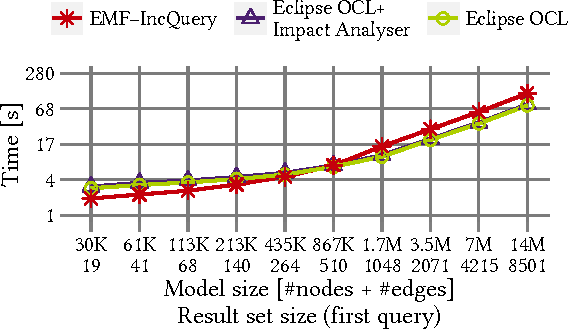
\includegraphics[width=0.9\textwidth]{figures/trainBenchmark_User_BatchValid_RouteSensor}
	    \caption{Batch Query Evaluation Time -- RouteSensor}
	    \label{fig:BatchValid_RouteSensor}
	\end{subfigure}
	\begin{subfigure}[t]{0.48\textwidth}\centering
	    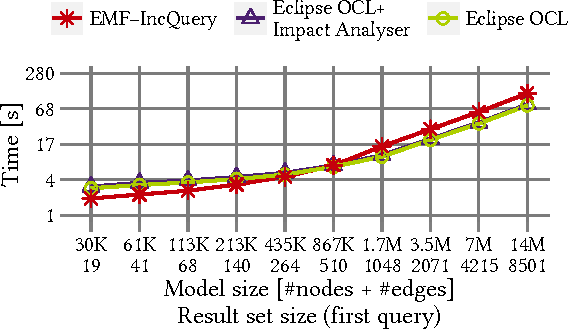
\includegraphics[width=0.9\textwidth]{figures/trainBenchmark_User_BatchValid_RouteSensor}
	    \caption{Batch Query Evaluation Time -- SignalNeighbor}
	    \label{fig:BatchValid_SignalNeighbor}
	\end{subfigure} \\

	\begin{subfigure}[t]{0.48\textwidth}\centering
	    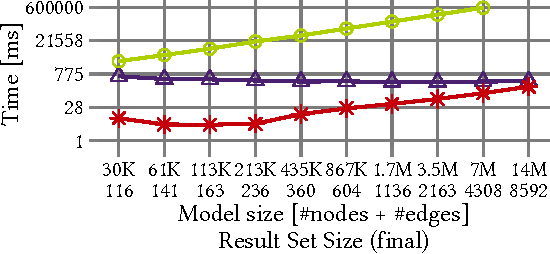
\includegraphics[width=0.9\textwidth]{figures/trainBenchmark_User_SumInc_RouteSensor}
	    \caption{Incremental Query Evaluation Time -- RouteSensor}
	    \label{fig:SumInc_RouteSensor}
	\end{subfigure}
	\begin{subfigure}[t]{0.48\textwidth}\centering
	    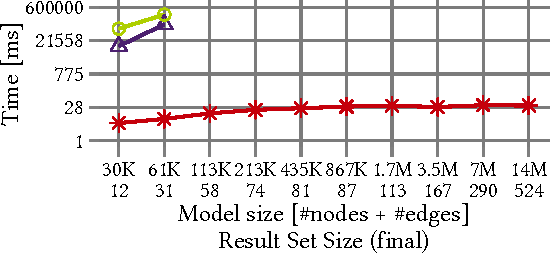
\includegraphics[width=0.9\textwidth]{figures/trainBenchmark_User_SumInc_SignalNeighbor}
	    \caption{Incremental Query Evaluation Time -- SignalNeighbor}
	    \label{fig:SumInc_SignalNeighbor}
	\end{subfigure} \\

	\begin{subfigure}[t]{0.48\textwidth}\centering
	    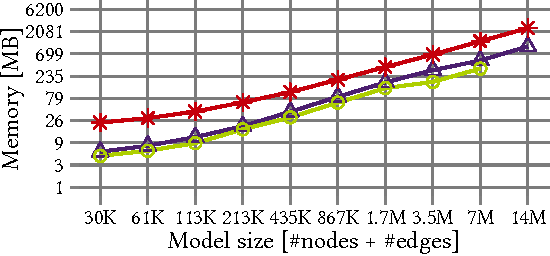
\includegraphics[width=0.9\textwidth]{figures/trainBenchmark_User_Memory_RouteSensor}
	    \caption{Memory Usage -- RouteSensor}
	    \label{fig:Memory_RouteSensor}
	\end{subfigure}
	\begin{subfigure}[t]{0.48\textwidth}\centering
	    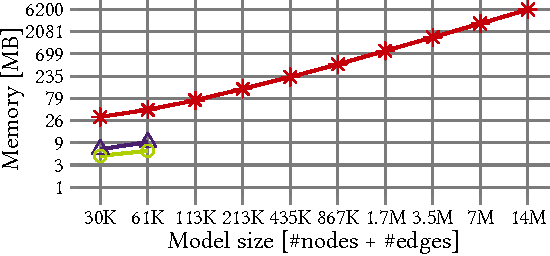
\includegraphics[width=0.9\textwidth]{figures/trainBenchmark_User_Memory_SignalNeighbor}
	    \caption{Memory Usage -- SignalNeighbor}
	    \label{fig:Memory_SignalNeighbor}
	\end{subfigure}
  \caption{Benchmark Results}
  \label{fig:trainbenchmark-diagrams}
\end{center}
\end{figure}

For the more complex \emph{SignalNeighbor} query
\autoref{fig:BatchValid_SignalNeighbor} depicts that \incquery{} (somewhat
surprisingly) outperforms OCL solutions: it is noticeably faster for small
modells ($2$s and $4$s), and over $435$k model elements OCL did not finish with
the initial analysis in $12$ minutes. This performance gain might be attributed to
the more efficient (cached) enumeration of instances, and the possibility of
backward navigation (with the help of auxiliary structures) on unidirectional
references used by this query.

\subsubsection{Incremental Query Evaluation}
In the \emph{incremental case}, Eclipse OCL evaluates the query on each issue
(i.e.\ : hundred times) from scratch, its execution time increases linearly with
model size, resulting slow overall evaluation.

For the \emph{RouteSensor} query (\autoref{fig:SumInc_RouteSensor}), the Impact
Analyzer performs the $100$ modifications in $350$ms regardless of the model
size. On the same query, \incquery{} starts much faster, but its speed reduces
on the larger models (from $9$ to $220$ms). On the other hand, the Impact
Analyzer is an order of magnitude slower on the \emph{SignalNeighbor} query
(\autoref{fig:SumInc_SignalNeighbor}) query: it does not finish in $12$ minutes
for models over $61$k model elements, while \incquery{} handles every model
regardless of size under $40$ms.

The performance of the Impact Analyzer is most likely affected by the previously
mentioned unidirectional references. The slowdown of \incquery{} is probably
caused by the increased number of matches (from $116$ to $8592$), as query
results are always available in the output nodes of Rete networks, and only a
linear traversal of these stored matches is needed to return them.

% is much faster, moreover performs its task in constant time.
% \incquery{} is faster than OCL Impact Analyser, but it somewhat increases for
% larger $x$ values. The evaluation time of the Rete based \incquery{} does not
% depend on model size, but on the notifications and result set size of output
% nodes (see \autoref{fig:incquery-rt-arch}). As in this testcase modifications
% are similar, this slight increase can be attributed to the change of the number
% of results from 141 to 8592. When the result sets does not vary much, it can
% return query results almost in constant time (be it a small or very large model)
% that is confirmed by \autoref{fig:SumInc_SignalNeighbor}. On the other hand,
% Eclipse OCL slows down and shows linear characteristics (as it is not an
% incremental solution), but interestingly, OCL Impact Analyzer behaves similarly.
% The Impact Analyzer is also orders of magnitude slower and the query evaluation
% time linearly increases as model size increases, perhaps due to the properties
% of the query described in the previous paragraph. In this case the OCL tests
% could be run only for the two smallest model, because for larger models the
% batch and incremental phases took in more than ten minutes resulting in timeout.

